\chapter{NLP}


% ---------- Bilingual Evaluation Understudy ----------
\clearpage
\thispagestyle{nlpstyle}
\section{BLEU}
\subsection{Bilingual Evaluation Understudy}
% references:
% https://aclanthology.org/P02-1040.pdf



BLEU is one of the earliest and most widely used metrics for evaluating machine translation and other
text generation tasks. It measures how similar a machine-generated text is to one or more human
reference translations by calculating the overlap of n-grams (contiguous sequences of words).

% equation
\begin{center}
    \tikz{
        \node[inner sep=2pt, font=\Large] (a) {
            {
                $\displaystyle
                BLEU = {\color{nmlred}BP} \cdot \exp\left(\sum_{n=1}^{N} {\color{nmlpurple}w_n} \log {\color{nmlcyan}p_n}\right)
                $
            }
        };
        \draw[overlay,-latex,nmlred, semithick] ($(a.south)+(-1.5,0.3)$) to[bend left=15] node[pos=1, left] {brevity penalty} +(-1,-.5);
        \draw[overlay,-latex,nmlcyan, semithick] ($(a.north)+(2.5,-0.2)$) to[bend left=15] node[pos=1, right] {n-gram precision} +(1,.5);
        \draw[overlay,-latex,nmlpurple, semithick] ($(a.south)+(1.0,0.3)$) to[bend right=15] node[pos=1, right] {n-gram weights} +(1,-.5);
    }
\end{center}

BLEU ranges from 0 to 1, where 1 indicates a perfect match with the reference.

\textbf{When to use BLEU?}

Use BLEU when evaluating machine translation, summarization, or text generation models where direct
word or phrase overlap with human-produced references is important.

\coloredboxes{
\item Correlates with human judgments at the corpus level. In its original study, BLEU showed strong
alignment with human evaluators.
\item Supports multiple references. Several human translations can be used, helping BLEU capture
natural variability.
\item To prevent models from producing unrealistically short outputs, BLEU introduces a
brevity penalty.
}
{
\item Insensitive to meaning. BLEU measures surface-level word overlap and does not account for
semantic equivalence.
\item Vulnerable to synonyms and paraphrasing. Valid alternative phrasings are not rewarded.
\item Sensitive to tokenization and normalization choices. BLEU scores can vary depending on how words
are segmented (e.g., handling of punctuation, casing, or subword units).
}

\clearpage

\thispagestyle{customstyle}

\begin{figure*}[ht!]
    \centering
    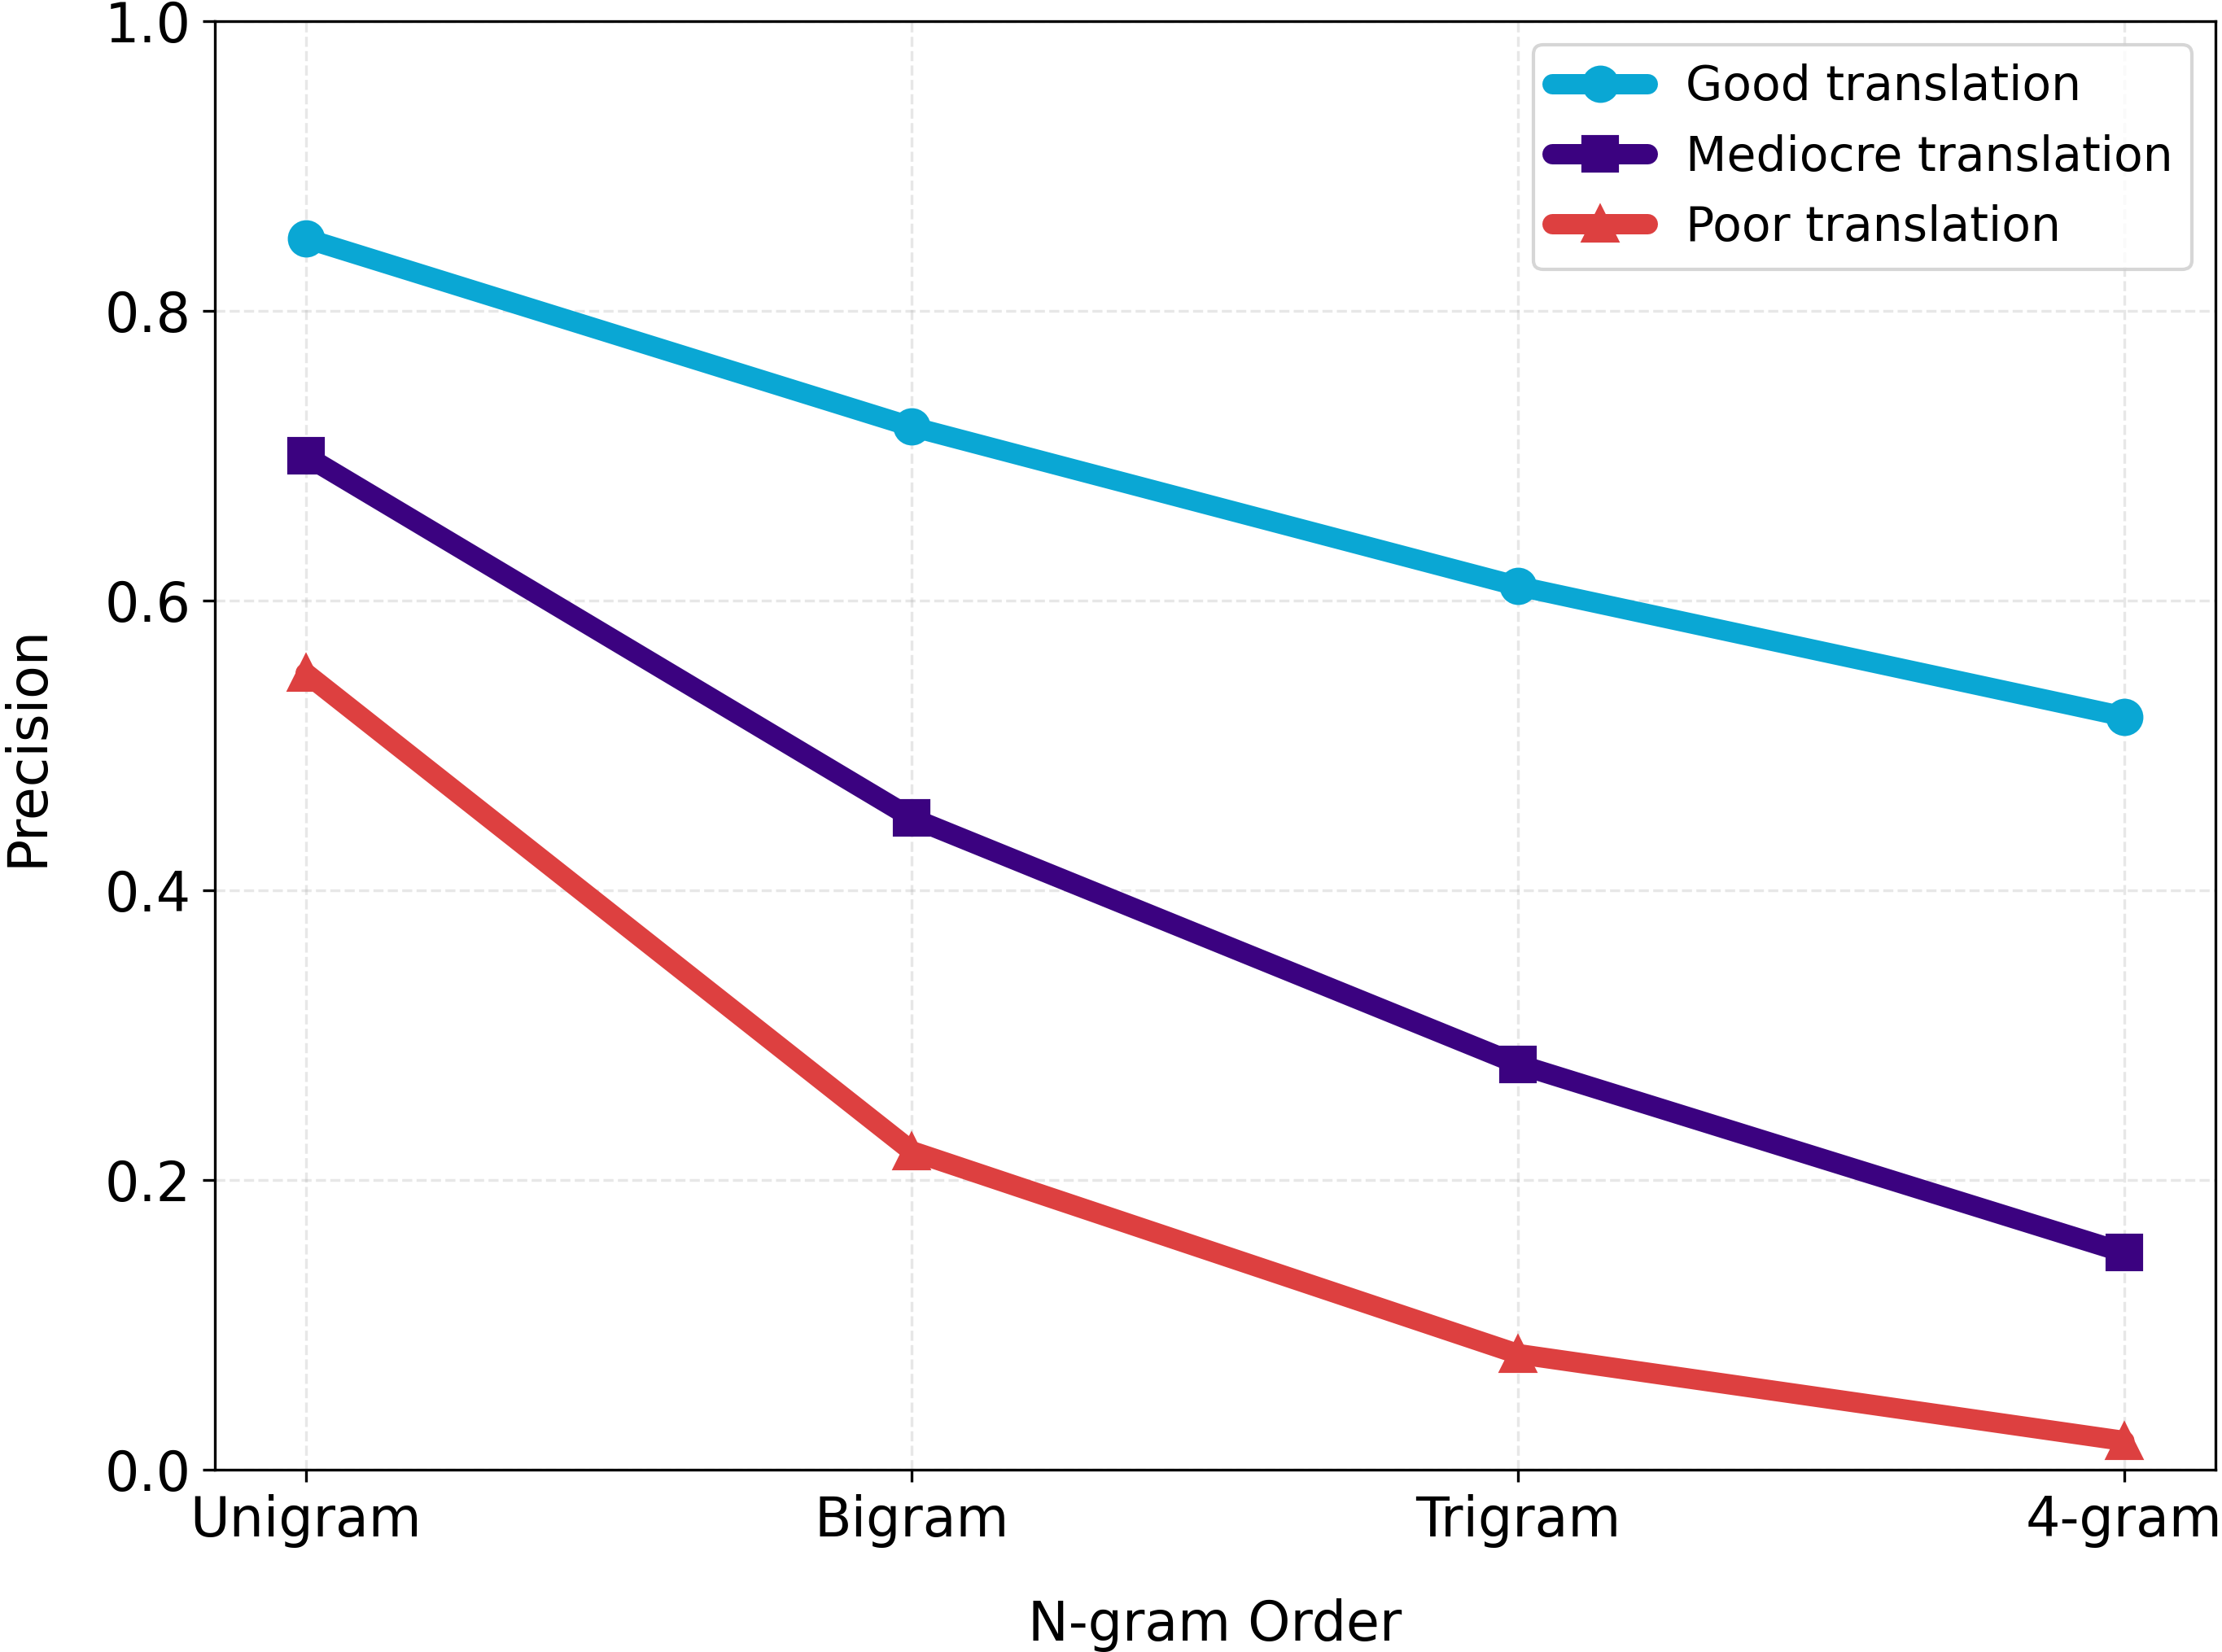
\includegraphics[width=0.6\textwidth]{figures/BLEU_ngram_precision.png}
\end{figure*}

\textbf{Figure.} N-gram precision drops as n increases. Good translations maintain high precision across all n-gram orders, while poor translations collapse at higher orders where exact phrase matches become rare.

\orangebox{Did you know that...}
{BLEU was introduced in 2002 by Papineni et al. at IBM and was the first automatic metric to gain
wide acceptance in machine translation research.}

\textbf{Other related metrics}

METEOR addresses BLEU's limitations with synonym matching and stemming. ROUGE focuses on recall rather than precision.
For learned semantic similarity, see BERTScore in the GenAI chapter.

% ---------- Metric for Evaluation of Translation with Explicit ORdering ----------
% references:
% https://aclanthology.org/W05-0909.pdf

\clearpage
\thispagestyle{nlpstyle}
\section{METEOR}
\subsection{Metric for Evaluation of Translation with Explicit ORdering}

METEOR (Metric for Evaluation of Translation with Explicit ORdering) is a machine translation
evaluation metric introduced as an improvement over BLEU. Unlike BLEU, which relies heavily on
exact n-gram matches, METEOR aligns candidate translations with reference translations using stemming,
synonyms, and paraphrases. 

% equation
\begin{center}
    \tikz{
        \node[inner sep=2pt, font=\Large] (a) {
            {
                $\displaystyle
                METEOR = (1 - {\color{nmlred}\gamma} \cdot {\color{nmlpurple}frag}^{\beta}) \cdot {\color{nmlcyan}F_{mean}}
                $
            }
        };
        \draw[overlay,-latex,nmlcyan, semithick] ($(a.north)+(2.5,-0.2)$) to[bend left=15] node[pos=1, right] {harmonic mean} +(1,.5);
        \draw[overlay,-latex,nmlpurple, semithick] ($(a.south)+(0.5,0.3)$) to[bend left=15] node[pos=1, left] {fragmentation penalty} +(-1,-.5);
    }
\end{center}

It then computes a harmonic mean of unigram precision and recall, with
recall weighted higher to better capture adequacy. Finally, it introduces a fragmentation penalty to
account for word order, rewarding translations that are both accurate and fluent.

\textbf{When to use METEOR?}

It is especially valuable when translation adequacy (capturing meaning) is as important as fluency.
Because it incorporates linguistic resources such as stemming and synonyms, METEOR is useful for
low-resource or morphologically rich languages, where exact matches are too strict.

\coloredboxes{
\item Closer to human judgment. METEOR was shown to correlate better with human evaluations compared
to BLEU.
\item Flexible matching. Accounts for stemming, synonyms, and paraphrases, making it more tolerant
to variation in expression.
\item Balances adequacy and fluency. By combining precision, recall, and word order penalties,
it reflects both meaning preservation and readability.
}
{
\item Computationally heavy. Requires linguistic resources (stemming, synonym databases),
making it slower than purely statistical metrics.
\item Language dependence. Its quality depends on the availability and completeness of stemming
rules and synonym dictionaries for the target language.
}

\clearpage

\thispagestyle{customstyle}

\begin{figure*}[ht!]
    \centering
    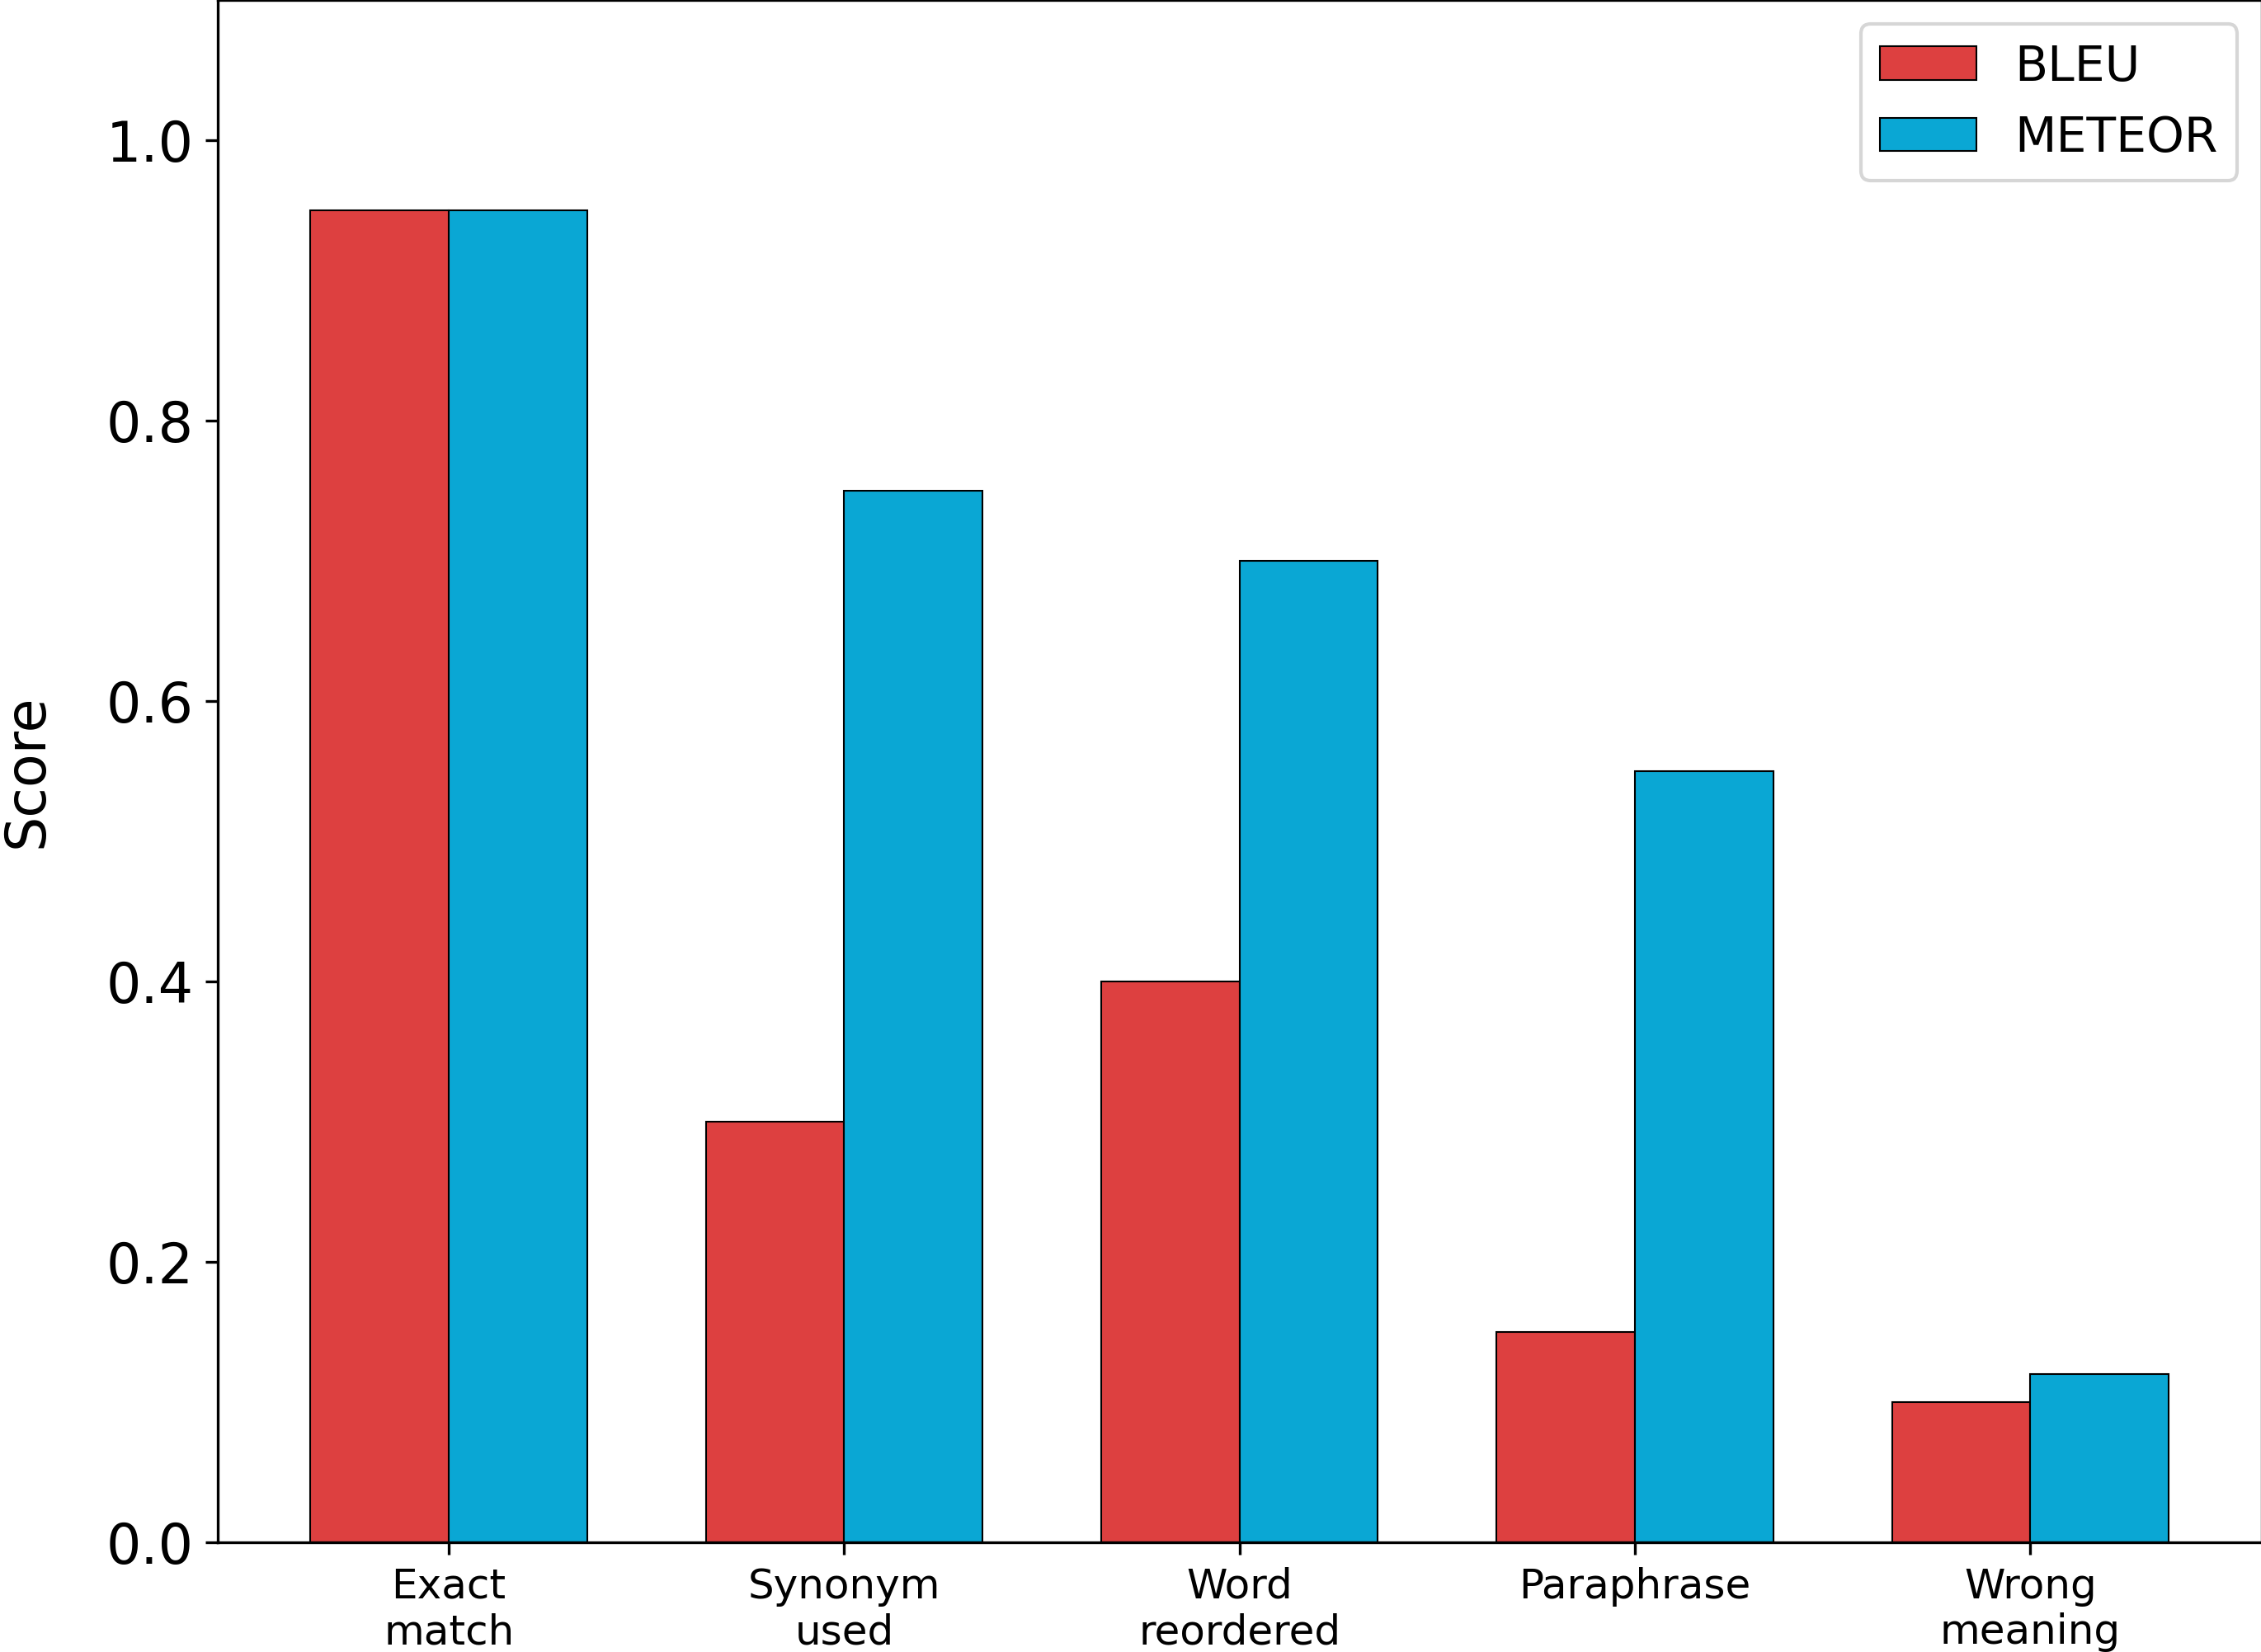
\includegraphics[width=0.6\textwidth]{figures/METEOR_vs_BLEU.png}
\end{figure*}

\textbf{Figure.} METEOR vs BLEU across different translation scenarios. METEOR rewards synonyms and paraphrases that BLEU misses, giving a more nuanced evaluation.

\orangebox{Did you know that...}
{METEOR was developed at Carnegie Mellon University in 2005 as a direct response to BLEU’s shortcomings.}

\textbf{Other related metrics}

METEOR improves on BLEU by incorporating synonyms and stemming. For recall-focused evaluation, see ROUGE.
For edit-distance-based evaluation, see TER.

% ---------- Recall-Oriented Understudy for Gisting Evaluation ----------
% references:
% https://aclanthology.org/W04-1013.pdf
% https://aclanthology.org/E17-2007.pdf

\clearpage
\thispagestyle{nlpstyle}
\section{ROUGE}
\subsection{Recall-Oriented Understudy for Gisting Evaluation}

ROUGE is a family of metrics designed to evaluate automatic summarization and machine translation by
comparing the overlap between a system-generated text and one or more reference texts.
Unlike precision-oriented measures, ROUGE emphasizes recall, how much of the important content from
the reference is captured by the system output.

% equation
\begin{center}
    \tikz{
        \node[inner sep=2pt, font=\Large] (a) {
            {
                $\displaystyle
                ROUGE\text{-}N = \frac{\sum_{s \in Ref} \sum_{gram_n \in s} {\color{nmlcyan}Count_{match}}(gram_n)}{\sum_{s \in Ref} \sum_{gram_n \in s} {\color{nmlpurple}Count}(gram_n)}
                $
            }
        };
        \draw[overlay,-latex,nmlcyan, semithick] ($(a.north)+(2.0,-0.1)$) to[bend left=15] node[pos=1, right] {matching n-grams} +(1,.5);
        \draw[overlay,-latex,nmlpurple, semithick] ($(a.south)+(2.0,0.3)$) to[bend left=15] node[pos=1, left] {total reference n-grams} +(-1,-.5);
    }
\end{center}

ROUGE scores range between 0 and 1, with higher values indicating higher similarity between the
system-generated text and the reference.

\textbf{When to use ROUGE?}

ROUGE is widely used in text summarization, where recalling important phrases is crucial, in machine
translation evaluation, and in other generation tasks such as captioning or dialogue, when
benchmarking against human-written references.

\coloredboxes{
\item Easy to compute and understand.
\item Many flexible variants available: ROUGE-N, ROUGE-L, and ROUGE-S capture different linguistic
overlaps (local n-grams, subsequences, or flexible structures).
}
{
\item ROUGE relies on lexical overlap and often misses semantic similarity.
\item Some studies have found that even human-written summaries can score poorly under ROUGE.
}

\clearpage

\thispagestyle{customstyle}

\begin{figure*}[ht!]
    \centering
    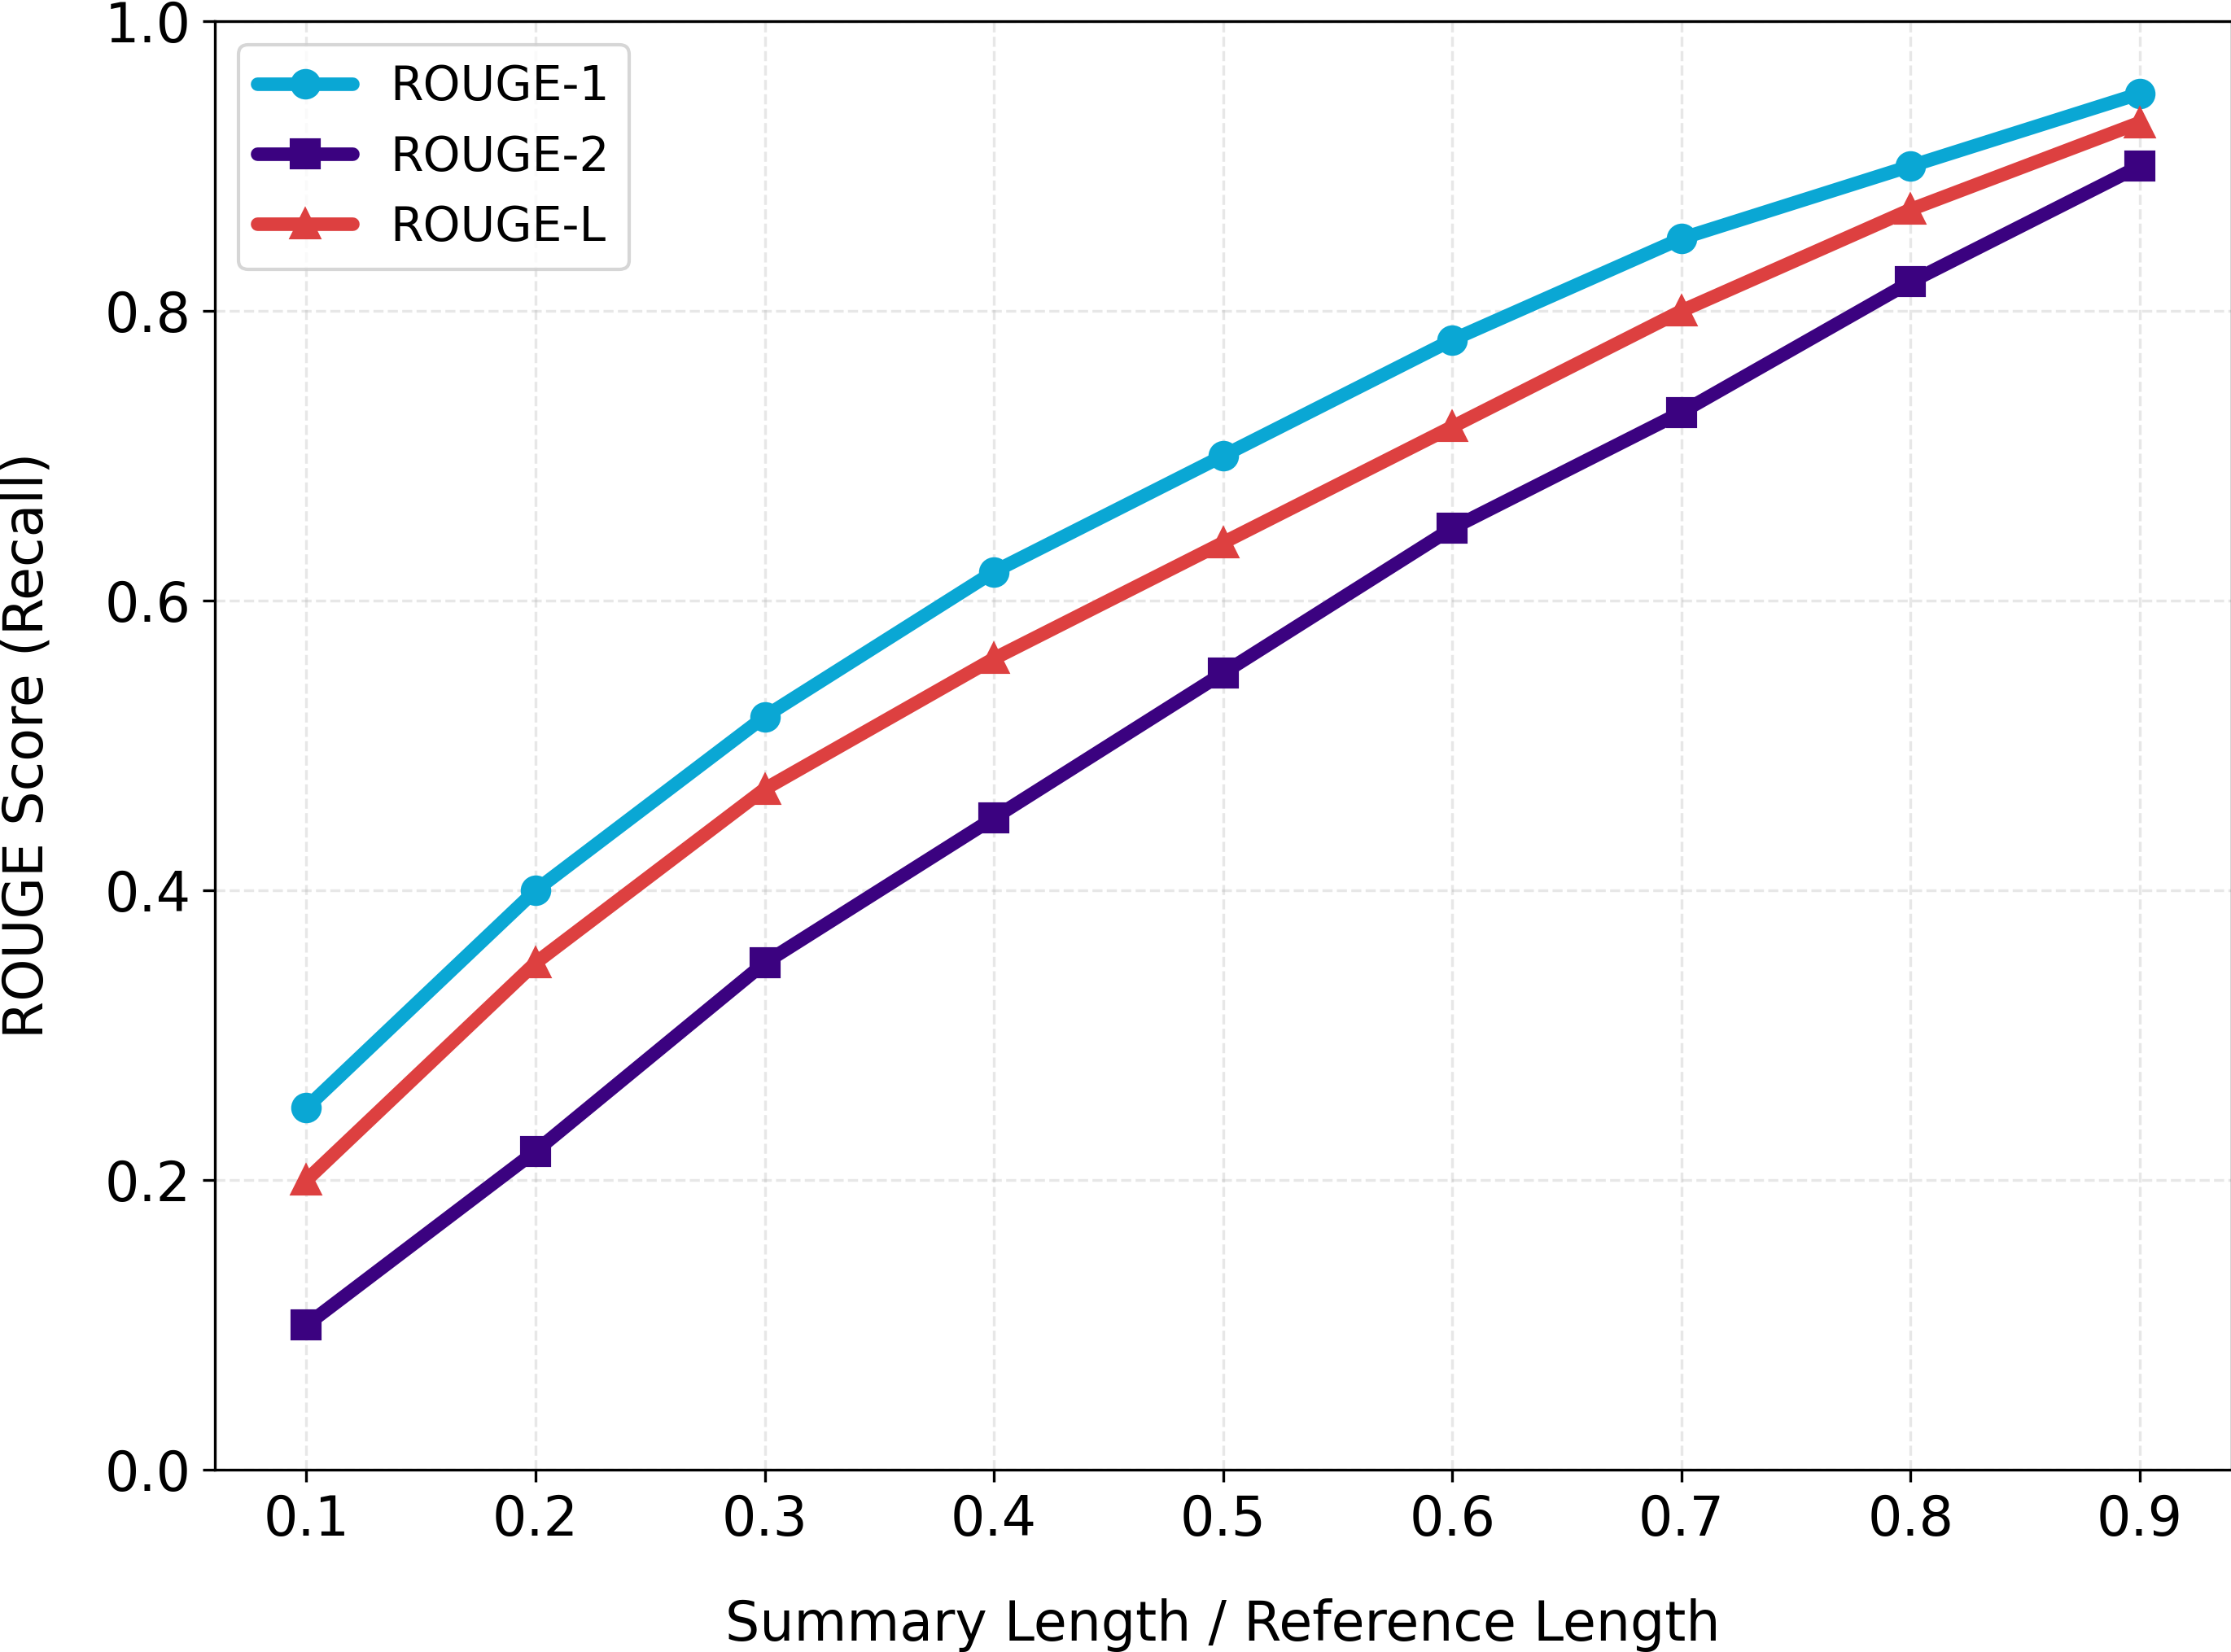
\includegraphics[width=0.6\textwidth]{figures/ROUGE_variants.png}
\end{figure*}

\textbf{Figure.} ROUGE recall scores increase as summary length approaches the reference length. ROUGE-1 (unigram) is highest, ROUGE-2 (bigram) lowest, and ROUGE-L (longest common subsequence) falls in between.

\orangebox{Did you know that...}
{ROUGE was introduced by Chin-Yew Lin in 2004 and quickly became a popular benchmark in text
summarization challenges. Despite its limitations, it is still one of the most reported
metrics in NLP.}

\textbf{Other related metrics}

ROUGE variants include ROUGE-N (n-gram overlap), ROUGE-L (longest common subsequence), and ROUGE-S (skip-bigram).
For precision-focused evaluation, use BLEU. For semantic similarity, see BERTScore.

% ---------- Translation Error Rate ----------
% reference: https://aclanthology.org/2006.amta-papers.25.pdf
\clearpage
\thispagestyle{nlpstyle}
\section{TER}
\subsection{Translation Error Rate}

TER is a metric designed to evaluate machine translation quality by measuring the number of edits
required to change a system’s translation into a reference translation. The edits include insertions,
deletions, substitutions, and shifts of word sequences.

% equation
\begin{center}
    \tikz{
        \node[inner sep=2pt, font=\Large] (a) {
            {
                $\displaystyle
                TER = \frac{{\color{nmlcyan}\text{insertions}} + {\color{nmlcyan}\text{deletions}} + {\color{nmlcyan}\text{substitutions}} + {\color{nmlpurple}\text{shifts}}}{{\color{nmlred}\text{reference length}}}
                $
            }
        };
        \draw[overlay,-latex,nmlcyan, semithick] ($(a.north)+(0.0,-0.1)$) to[bend right=15] node[pos=1, left] {word-level edits} +(-1,.5);
        \draw[overlay,-latex,nmlpurple, semithick] ($(a.north)+(3.0,-0.1)$) to[bend left=15] node[pos=1, right] {sequence shifts} +(1,.5);
        \draw[overlay,-latex,nmlred, semithick] ($(a.south)+(2.0,0.3)$) to[bend left=15] node[pos=1, left] {words in reference} +(-1,-.5);
    }
\end{center}

The score ranges from 0 to +infinity, where 0 indicates a perfect translation (no edits required).
Higher values correspond to translations needing more post-editing.

\textbf{When to use TER?}

Use TER when you want a metric that correlates closely with the amount of human editing effort
required to correct machine translations.

\coloredboxes{
\item Easy to compute and understand.
\item Includes word reordering (shifts), which captures errors that BLEU and related metrics
often miss.
}
{
\item Does not account for semantic equivalence when different but correct word choices are used.
\item TER tends to overestimate the actual translation error rate compared to human
post-editing effort.
}

\clearpage

\thispagestyle{customstyle}

\begin{figure*}[ht!]
    \centering
    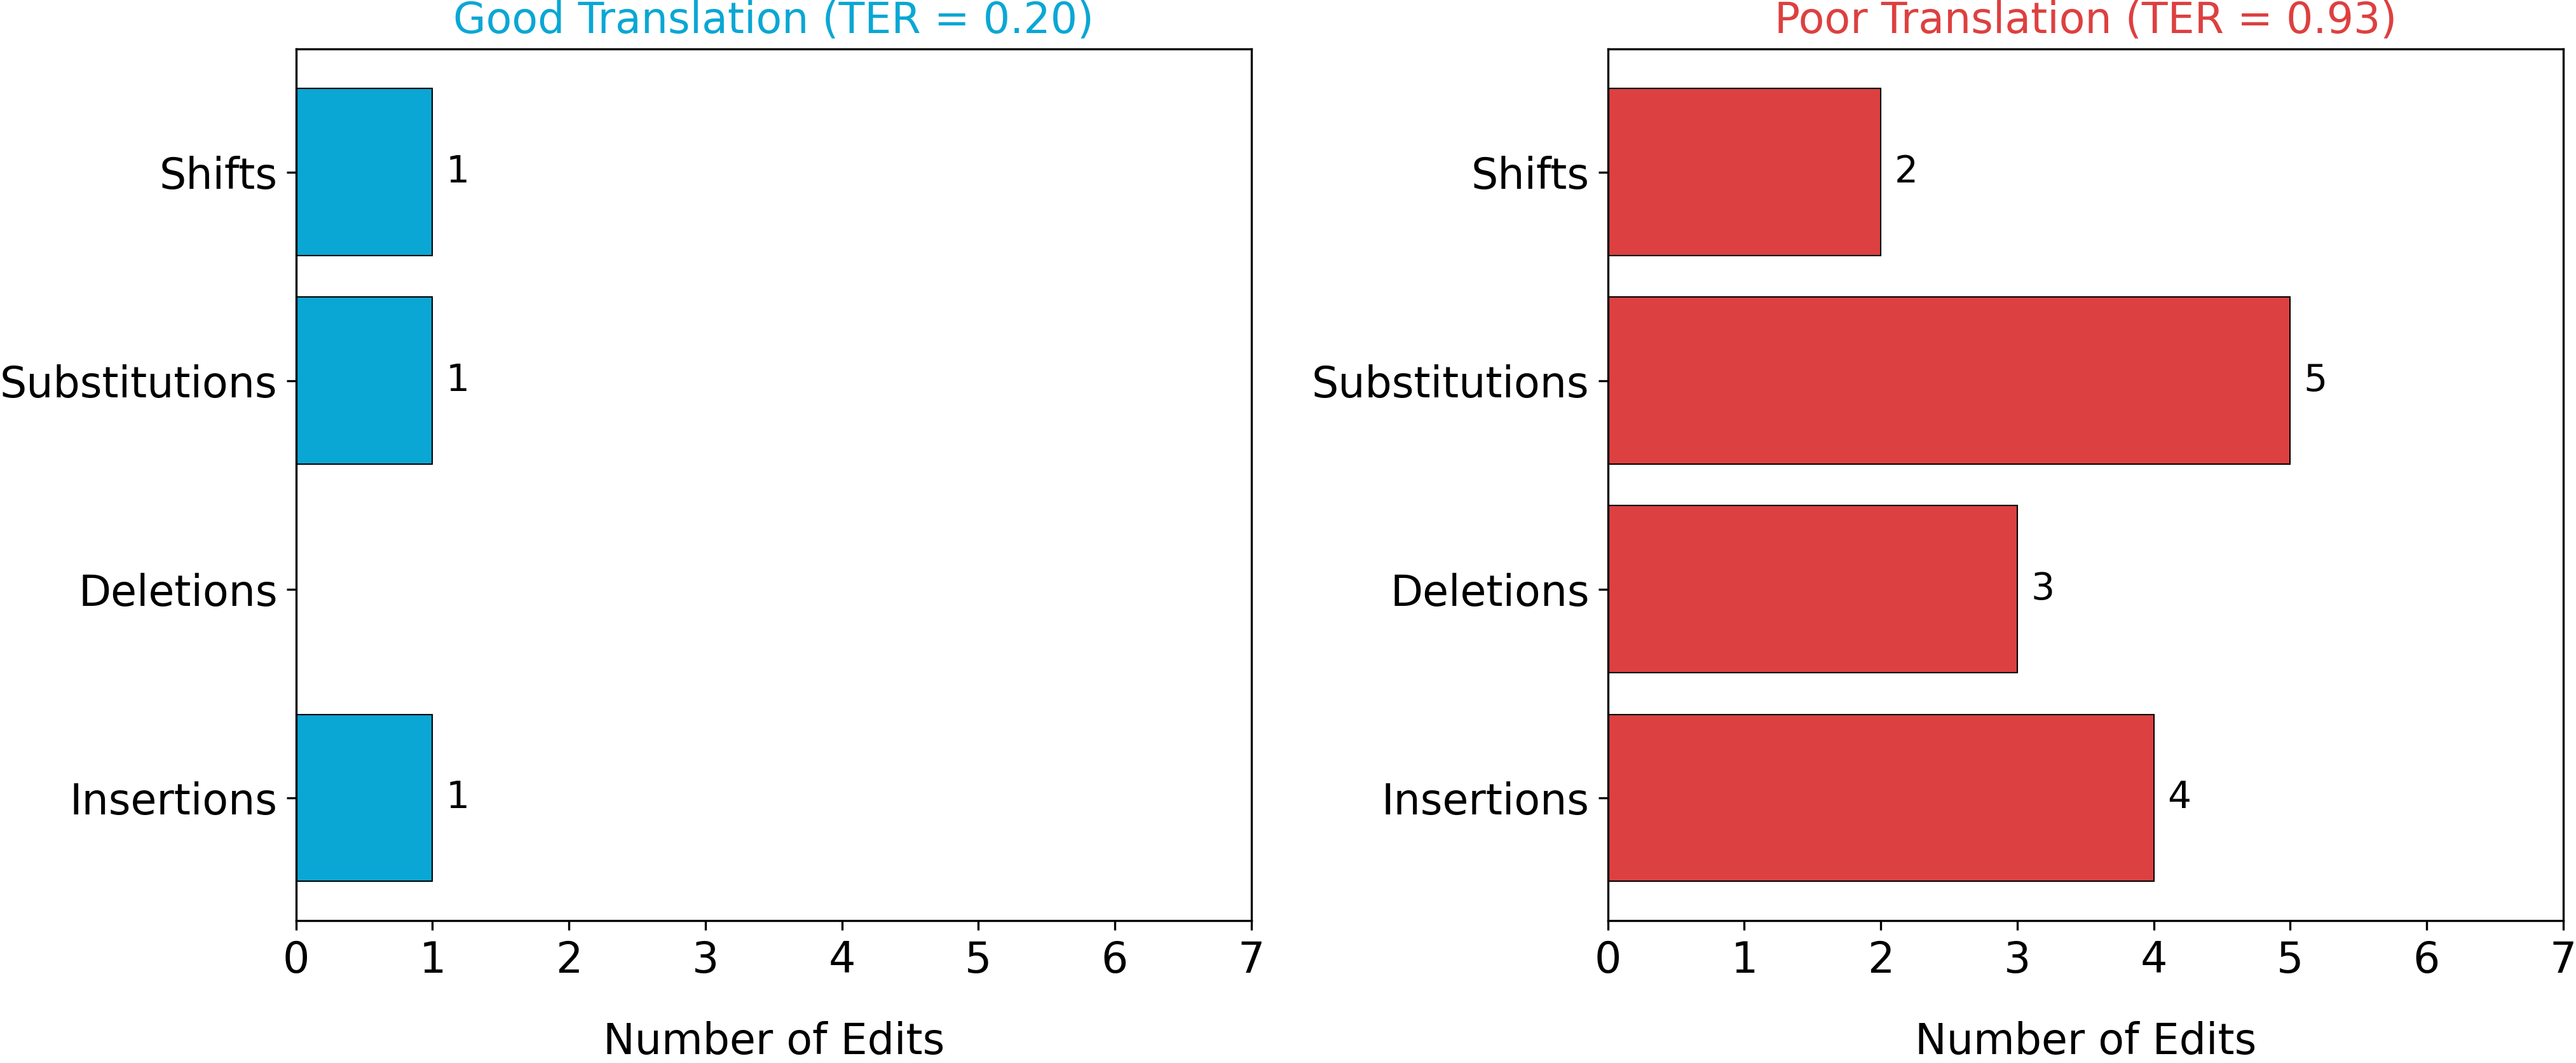
\includegraphics[width=\textwidth]{figures/TER_edit_breakdown.png}
\end{figure*}

\textbf{Figure.} Edit operation breakdown for good (TER=0.20) vs poor (TER=0.93) translations. A good translation requires minimal edits, while a poor one needs extensive substitutions, insertions, and deletions.

\orangebox{Did you know that...}
{TER was introduced by Snover et al. (2006) to provide a more human-centered evaluation of
machine translation.}

\textbf{Other related metrics}

TER is an edit-distance metric like WER but operates at the word level for translations. Unlike BLEU and METEOR,
lower TER is better. For speech recognition evaluation, see WER.

% ---------- Exact Match ----------
% reference: https://nlp.stanford.edu/pubs/rajpurkar2016squad.pdf
\clearpage
\thispagestyle{nlpstyle}
\section{EM}
\subsection{Exact Match}

Exact Match measures the percentage of predictions that exactly match the ground-truth answers,
word-for-word and character-for-character. The metric returns 1 if the predicted output is an
exact match with the reference text, and 0 otherwise. The overall score is the average across all
samples.

% equation
\begin{center}
    \tikz{
        \node[inner sep=2pt, font=\Large] (a) {
            {
                $\displaystyle
                EM = \frac{1}{{\color{nmlred}N}} \sum_{i=1}^{N} {\color{nmlgreen}\mathds{1}}({\color{nmlpurple}\hat{y}_i} = {\color{nmlcyan}y_i})
                $
            }
        };
        \draw[overlay,-latex,nmlred, semithick] ($(a.south)+(-0.5,0.2)$) to[bend left=15] node[pos=1, left] {number of samples} +(-1,-.5);
        \draw[overlay,-latex,nmlpurple, semithick] ($(a.north)+(1.0,-0.2)$) to[bend right=15] node[pos=1, left] {predicted text} +(-1,.5);
        \draw[overlay,-latex,nmlcyan, semithick] ($(a.north)+(1.9,-0.2)$) to[bend left=15] node[pos=1, right] {reference text} +(1,.5);
    }
\end{center}

EM is considered one of the strictest evaluation metrics since even a small deviation, such as an
extra space, different casing, or synonymous phrasing, leads to a score of 0.

\textbf{When to use EM?}

Use EM when exactness is critical. For instance, in extractive question answering, where the predicted
span must exactly match the gold answer. In structured outputs, such as JSON key-value generation,
where even a single mismatch makes the output invalid.

\coloredboxes{
\item Easy to calculate and explain. The prediction is either right or wrong.
\item Strict correctness guarantee. Particularly valuable when any deviation from the ground truth
is unacceptable (e.g., API calls, database queries).
}
{
\item Overly rigid. Does not account for semantically equivalent answers.
\item Not suitable for open-ended generation.
}

\clearpage

\begin{figure*}[ht!]
    \centering
    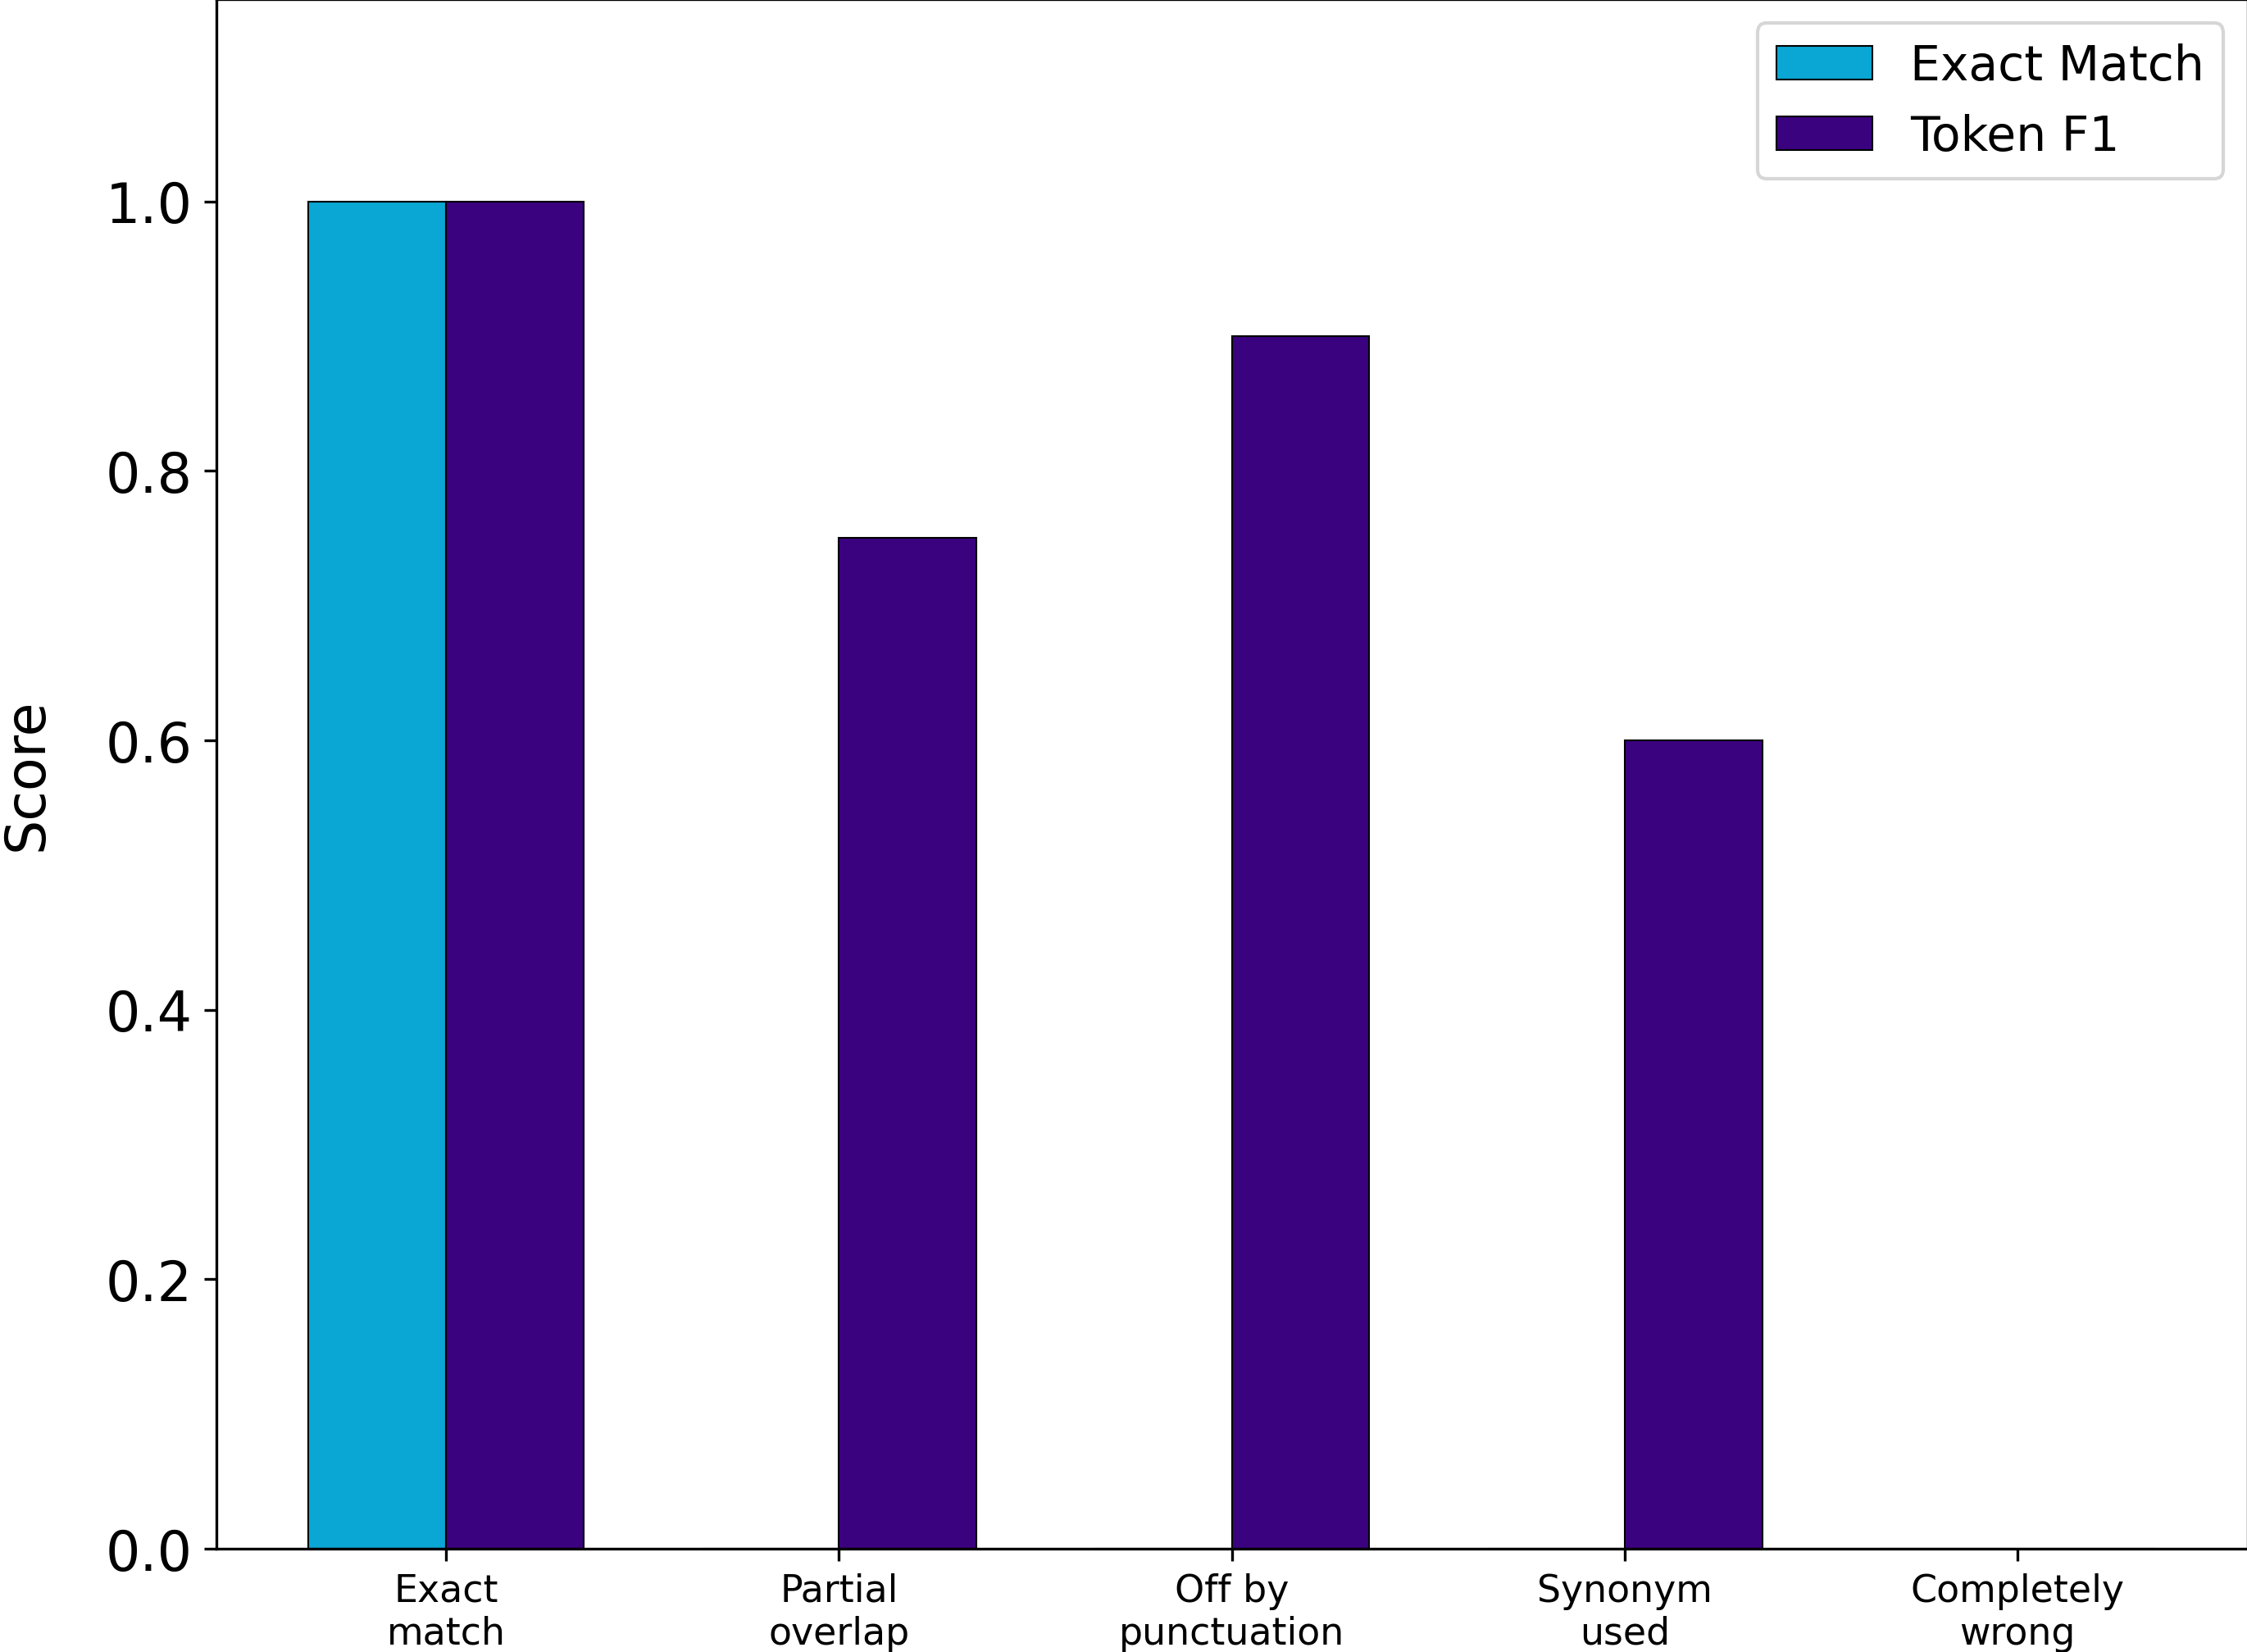
\includegraphics[width=0.6\textwidth]{figures/EM_vs_F1.png}
\end{figure*}

\textbf{Figure.} EM vs Token F1 across different answer types. EM gives zero credit for partial matches, synonyms, or punctuation differences, while Token F1 provides partial credit.

\orangebox{Did you know that...}
{Exact Match is one of the core metrics used in the Stanford Question Answering Dataset (SQuAD)
benchmark. However, because it is so strict, researchers often report both EM and F1 score.
EM for exact correctness, and F1 to give partial credit when a prediction overlaps significantly with
the ground truth.}

\textbf{Other related metrics}

EM is the strictest text comparison metric. For partial credit, use token-level F1-score. For n-gram overlap, see BLEU or ROUGE.

% ---------- Word Error Rate ----------
\clearpage
\thispagestyle{nlpstyle}
\section{WER}
\subsection{Word Error Rate}

Word Error Rate (WER) is one of the most widely used metrics for evaluating the performance of automatic speech recognition (ASR) systems.
It measures the difference between the predicted transcription and the reference transcription by counting the minimum number of word-level edits
required to transform one into the other. These edits include insertions, deletions, and substitutions. The metric is normalized by the total number
of words in the reference.

% equation
\begin{center}
    \tikz{
        \node[inner sep=2pt, font=\Large] (a) {
            {
                $\displaystyle
                WER = \frac{{\color{nmlcyan}S} + {\color{nmlcyan}D} + {\color{nmlcyan}I}}{{\color{nmlred}N}}
                $
            }
        };
        \draw[overlay,-latex,nmlcyan, semithick] ($(a.north)+(0.5,-0.1)$) to[bend right=15] node[pos=1, left] {edit operations} +(-1,.5);
        \draw[overlay,-latex,nmlred, semithick] ($(a.south)+(1.0,0.2)$) to[bend left=15] node[pos=1, left] {words in reference} +(-1,-.5);
    }
\end{center}

A WER of 0 indicates a perfect transcription, while higher values mean more errors. Interestingly, WER can even exceed 1 if the number of insertions
and substitutions is very large relative to the reference length.

\textbf{When to use WER?}

WER is best used for evaluating ASR systems, voice-to-text tools, and spoken dialogue systems where accurate transcription is essential.

\coloredboxes{
\item It provides a clear and interpretable measure of how closely the system output matches the ground truth.
\item Fine-grained. Captures insertion, deletion, and substitution errors separately, providing diagnostic insight.
}
{
\item Insensitive to meaning. WER penalizes all errors equally, even if substitutions do not change the overall meaning of the sentence.
}

\clearpage

\begin{figure*}[ht!]
    \centering
    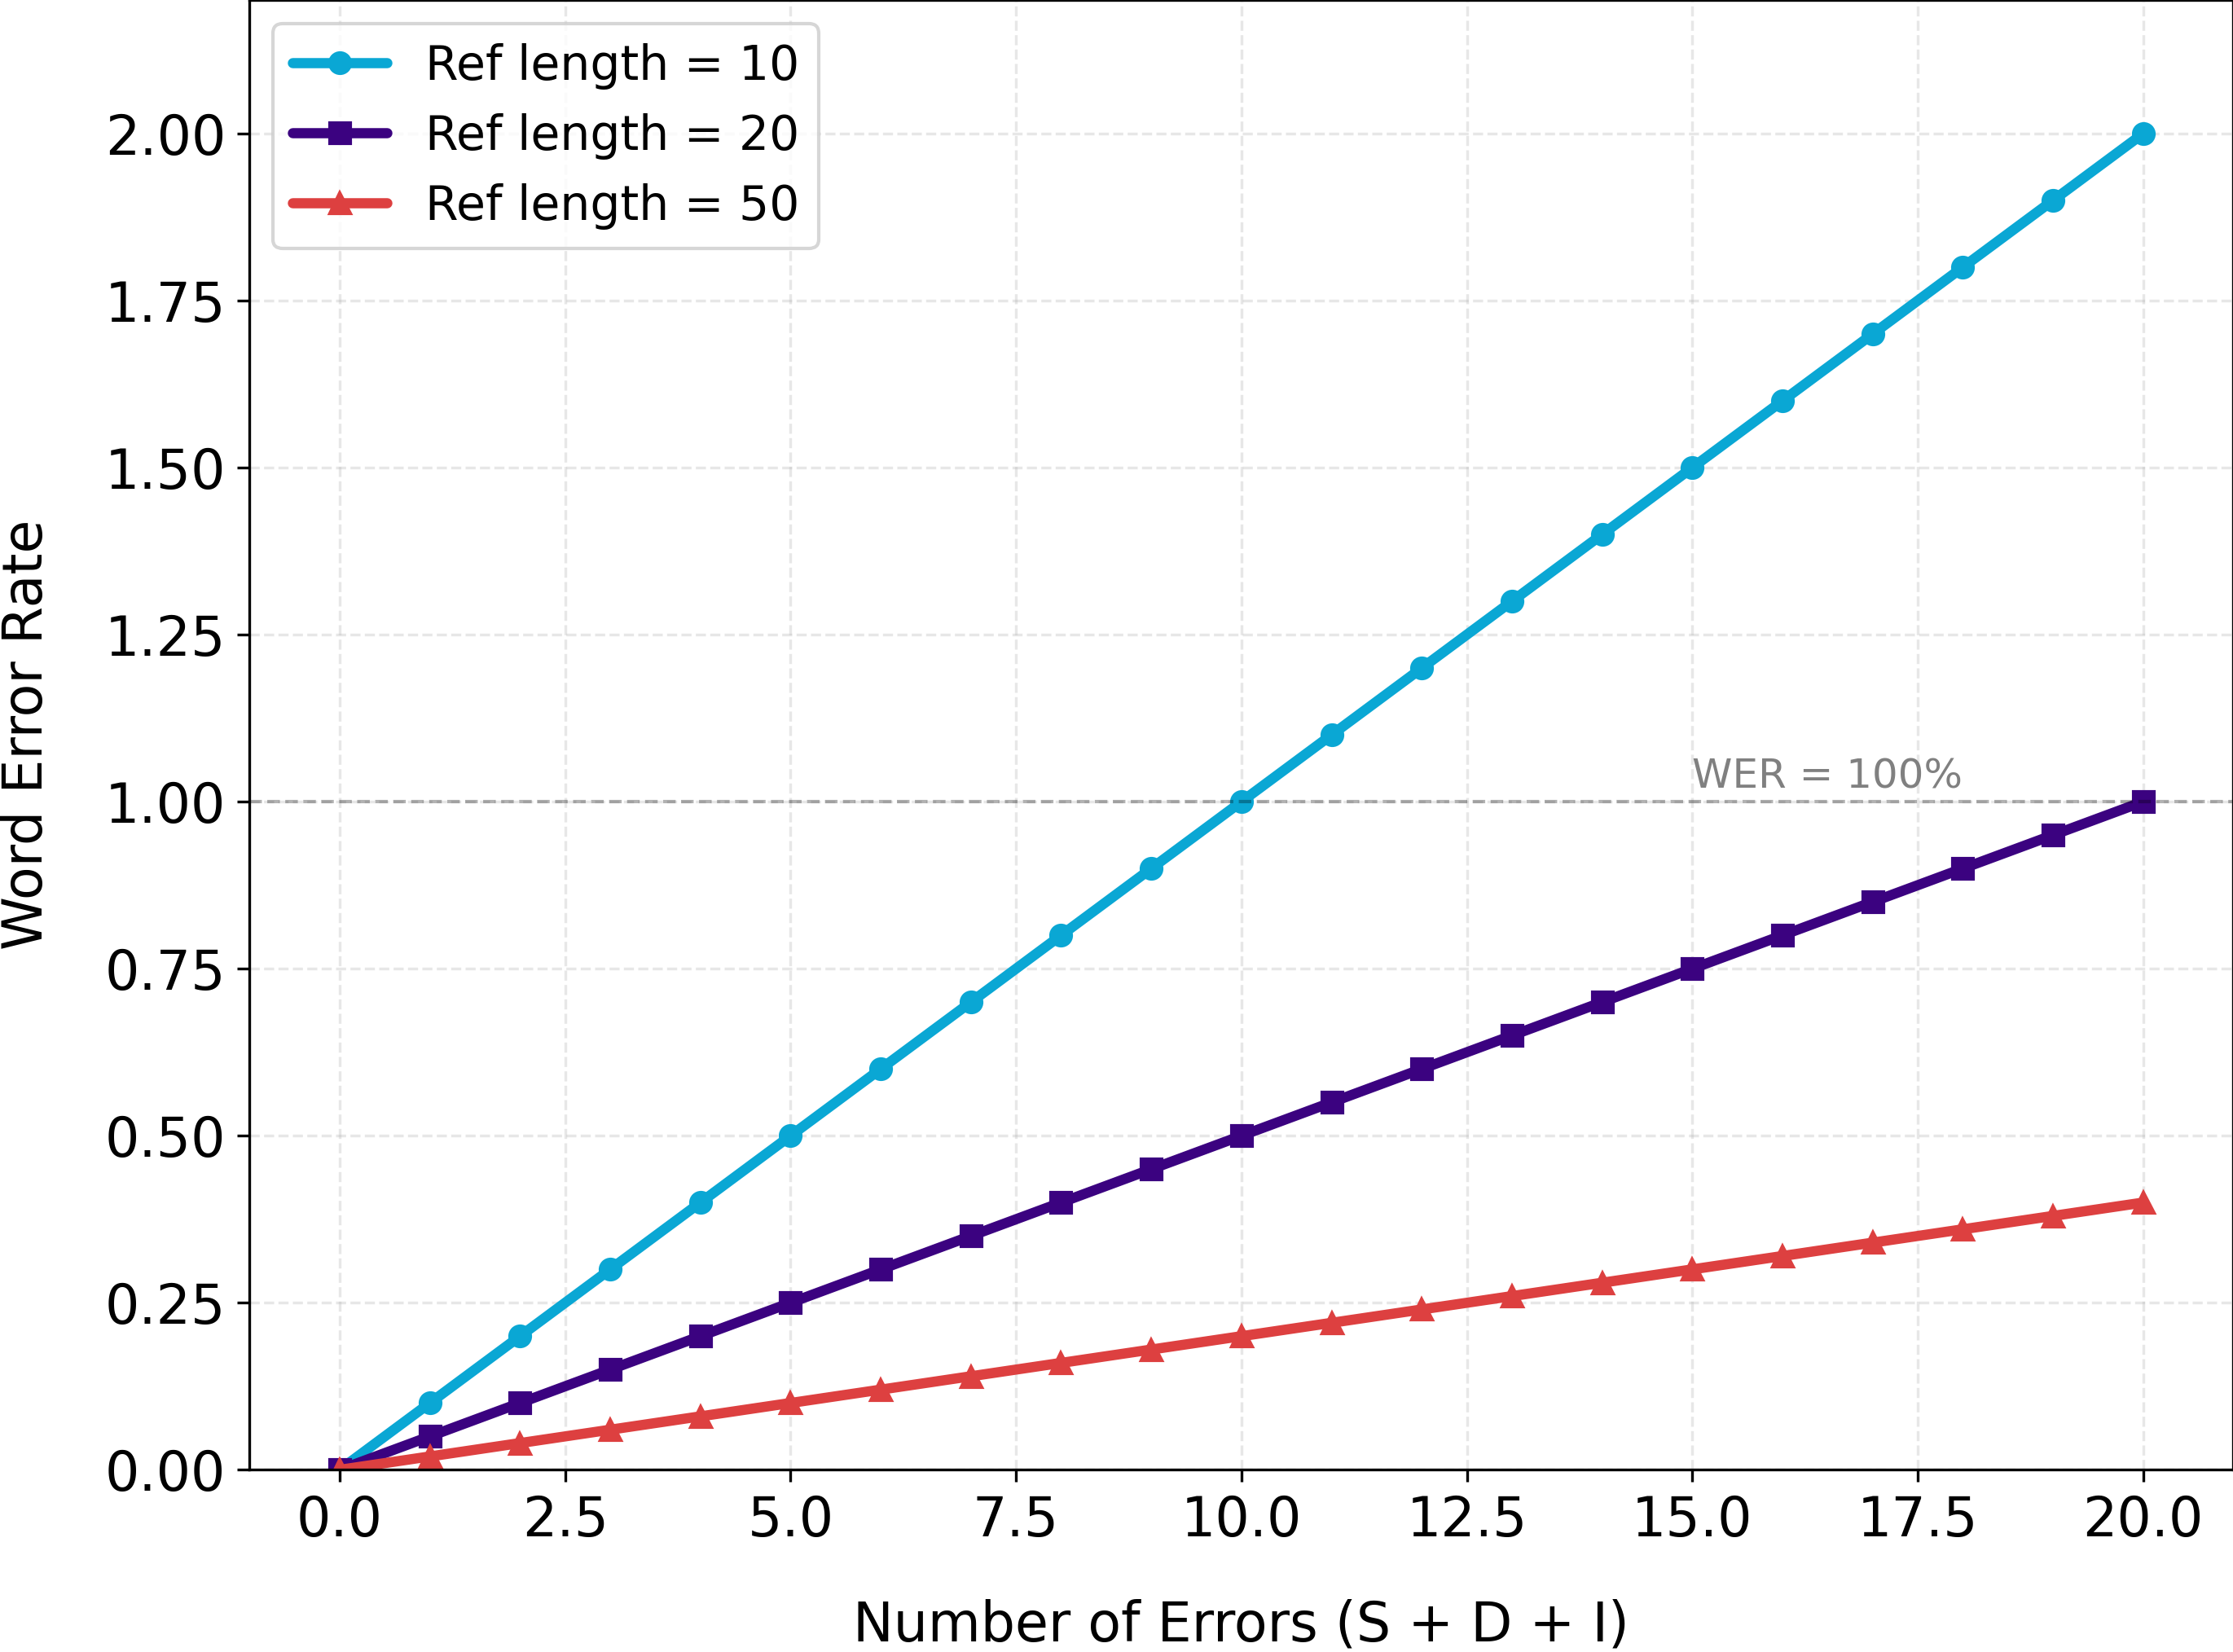
\includegraphics[width=0.6\textwidth]{figures/WER_vs_errors.png}
\end{figure*}

\textbf{Figure.} WER as a function of the number of errors for different reference lengths. Shorter references are more sensitive to each error. Note that WER can exceed 100\% when insertions outnumber reference words.

\orangebox{Did you know that...}
{Word Error Rate is essentially a specialized form of the Levenshtein distance, a string metric introduced in 1965 to measure how many
single-character edits are needed to transform one word into another. WER applies the same idea at the word level instead of characters,
counting insertions, deletions, and substitutions of words to compute the distance between the predicted and reference transcriptions.}

\textbf{Other related metrics}

WER is closely related to TER (Translation Error Rate), which adds word-sequence shifts as an edit operation. For character-level evaluation,
consider Character Error Rate (CER). For semantic evaluation beyond surface-level edits, see BERTScore.